\documentclass[tikz,border=8pt]{standalone}
% Shared look for every TikZ diagram. Load with \input{../../tools/tikz-style.tex}
\usepackage[sfdefault]{roboto}
\usetikzlibrary{arrows.meta, positioning, shapes.geometric, calc, fit, backgrounds}
\definecolor{cblue}{HTML}{4C78A8}
\definecolor{corange}{HTML}{F58518}
\definecolor{cgreen}{HTML}{54A24B}
\definecolor{cred}{HTML}{E45756}
\definecolor{cpurple}{HTML}{B279A2}
\definecolor{cgrey}{HTML}{6B6B6B}
\tikzset{
  every picture/.style={font=\sffamily, line width=1.2pt},
  box/.style={draw=#1, fill=#1!12, rounded corners=4pt, align=center, inner sep=7pt, minimum height=1.1cm},
  box/.default=cgrey,
  arrow/.style={-{Stealth[length=3mm]}, draw=cgrey, line width=1.4pt},
  title/.style={font=\sffamily\bfseries\Large},
  note/.style={font=\sffamily\small, text=cgrey, align=center},
}
\AtBeginDocument{\hyphenpenalty=10000 \exhyphenpenalty=10000}

% The order in which computeVelocityCommands() (src/teb_local_planner_ros.cpp, ros2-master) and
% HomotopyClassPlanner::plan() (src/homotopy_class_planner.cpp) run their steps; numbers are this Note's sections.
\begin{document}
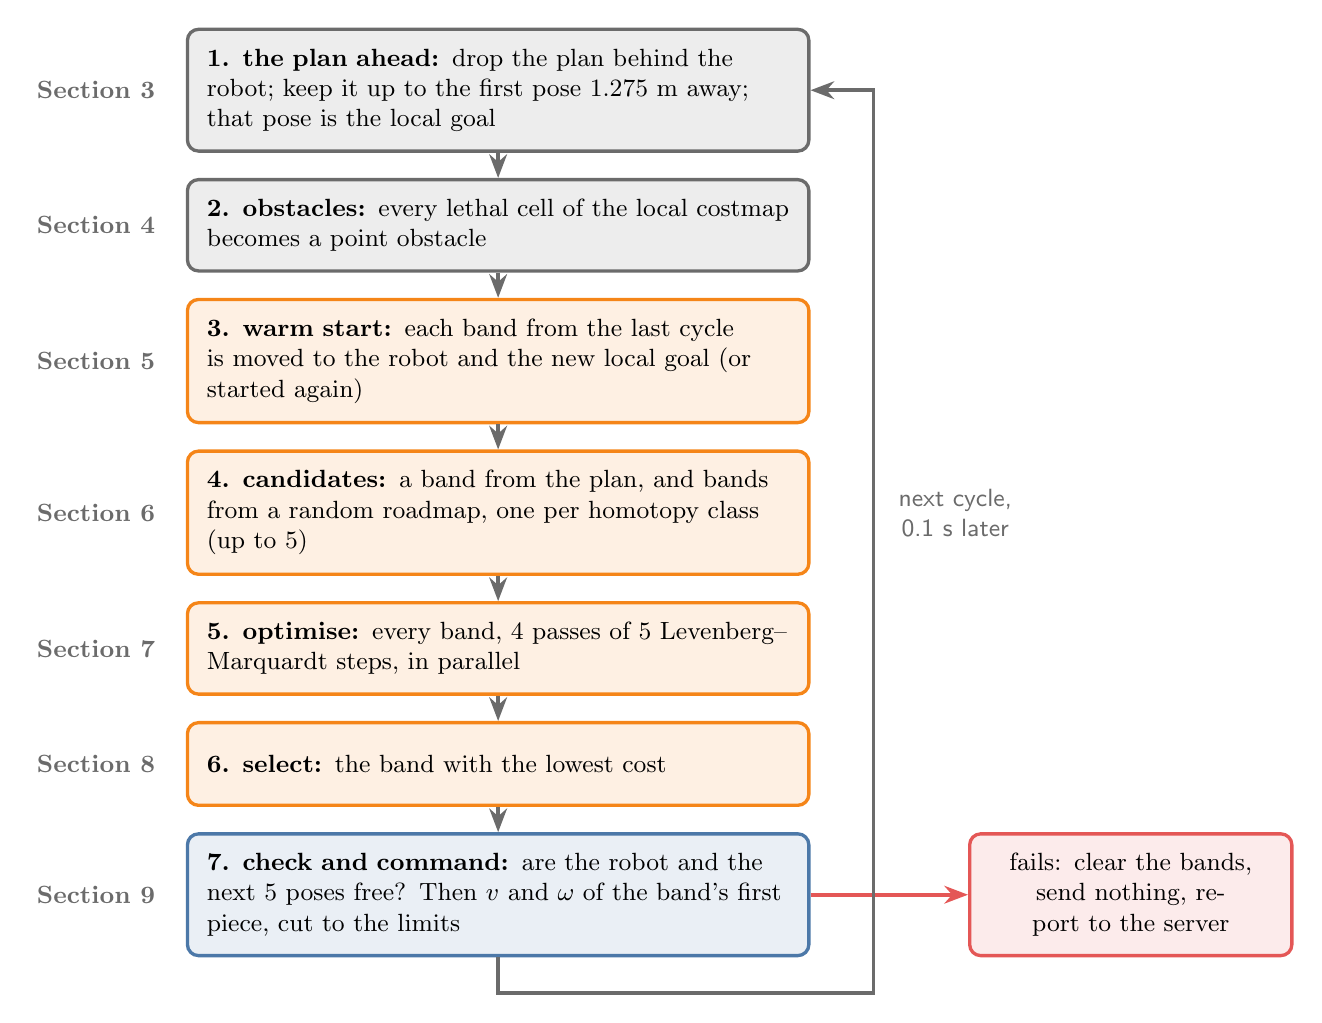
\begin{tikzpicture}[node distance=0.32cm,
  st/.style={box=#1, font=\small, text width=7.4cm, minimum height=1.05cm, align=left},
  sec/.style={font=\small\bfseries, text=cgrey, anchor=east}]
  \node[st=cgrey] (s1) {\textbf{1. the plan ahead:} drop the plan behind the robot; keep it up to the first pose 1.275 m away; that pose is the local goal};
  \node[st=cgrey, below=of s1] (s2) {\textbf{2. obstacles:} every lethal cell of the local costmap becomes a point obstacle};
  \node[st=corange, below=of s2] (s3) {\textbf{3. warm start:} each band from the last cycle is moved to the robot and the new local goal (or started again)};
  \node[st=corange, below=of s3] (s4) {\textbf{4. candidates:} a band from the plan, and bands from a random roadmap, one per homotopy class (up to 5)};
  \node[st=corange, below=of s4] (s5) {\textbf{5. optimise:} every band, 4 passes of 5 Levenberg--Marquardt steps, in parallel};
  \node[st=corange, below=of s5] (s6) {\textbf{6. select:} the band with the lowest cost};
  \node[st=cblue, below=of s6] (s7) {\textbf{7. check and command:} are the robot and the next 5 poses free? Then $v$ and $\omega$ of the band's first piece, cut to the limits};
  \foreach \a/\b in {s1/s2, s2/s3, s3/s4, s4/s5, s5/s6, s6/s7} \draw[arrow] (\a) -- (\b);
  \node[sec] at ([xshift=-0.25cm]s1.west) {Section 3};
  \node[sec] at ([xshift=-0.25cm]s2.west) {Section 4};
  \node[sec] at ([xshift=-0.25cm]s3.west) {Section 5};
  \node[sec] at ([xshift=-0.25cm]s4.west) {Section 6};
  \node[sec] at ([xshift=-0.25cm]s5.west) {Section 7};
  \node[sec] at ([xshift=-0.25cm]s6.west) {Section 8};
  \node[sec] at ([xshift=-0.25cm]s7.west) {Section 9};
  \node[box=cred, font=\small, text width=3.6cm, right=2.0cm of s7] (f) {fails: clear the bands, send nothing, report to the server};
  \draw[arrow, draw=cred] (s7) -- (f);
  \draw[arrow] (s7.south) -- ++(0,-0.45) -| ([xshift=0.8cm]s1.east |- s7.south) |- (s1.east);
  \node[note, text width=1.6cm, anchor=west] at ([xshift=0.9cm]s4.east) {next cycle, 0.1 s later};
\end{tikzpicture}
\end{document}
